\documentclass[answers]{exam}
\makeindex

\usepackage{amsmath, amsfonts, amssymb, amstext, amscd, amsthm, makeidx, graphicx, hyperref, url, enumerate}
\newtheorem{theorem}{Theorem}
\allowdisplaybreaks

\begin{document}

\begin{center}
{\Large CS 156a - Problem Set 5} \\
\medskip
Marco Yang \\
\medskip
2237027
\bigskip
\end{center}

\section*{Linear Regression Error}

Consider a noisy target \( y = \textbf{w*}^T x + \epsilon \), where 
\( \textbf{x} \in \mathbb{R}^d \) (with the added coordinate \( x_0 = 1 \)), 
\( y \in \mathbb{R} \), \( \textbf{w*} \) is an unknown vector, and \( \epsilon \) 
is a noise term with zero mean and \( \sigma^2 \) variance. Assume \( \epsilon \) 
is independent of \( \textbf{x} \) and of all other \( \epsilon \) values. If 
linear regression is carried out using a training data set $\mathcal{D}=
\{(\textbf{x}_{1}, y), \ldots, (\textbf{x}_{N}, y_{N})\}$, and outputs the 
parameter vector $\textbf{w}_{\text{lin}}$, it can be shown that the expected
in-sample error $E_{\text{in}}$ w.r.t. $\mathcal{D}$ is given by

\[
\mathbb{E}_\mathcal{D}[E_{\text{in}}(\textbf{w}_{\text{lin}})] = \sigma^2 \left(1 - \frac{d+1}{N}\right)
.\]

\begin{questions}

\question 
For \( \sigma = 0.1 \) and \( d = 8 \), which choice is the smallest number of
samples \( N \) that will result in an expected \( E_{\text{in}} > 0.008 \)?

\begin{choices}
    \choice 10
    \choice 25
    \choice 100
    \choice 500
    \choice 1000
\end{choices}

\begin{solution}
C. 100.

\[
0.1^2\left( 1 - \frac{9}{N} \right) > 0.08 \implies N > 45
.\] 
\end{solution}

\end{questions}

\section*{Nonlinear Transforms}

In linear classification, consider the feature transform 
\( \Phi: \mathbb{R}^2 \rightarrow \mathbb{R}^2 \) (plus the added coordinate) 
given by:

\[
\Phi(1, x_1, x_2) = (1, x_1^2, x_2^2)
\]

\begin{questions}
\setcounter{question}{1}

\question 
Which set of constraints on the weights in \( \mathcal{Z} \) space could 
correspond to the hyperbolic decision boundary in \( \mathcal{X} \) depicted
in the figure?

\begin{center}
    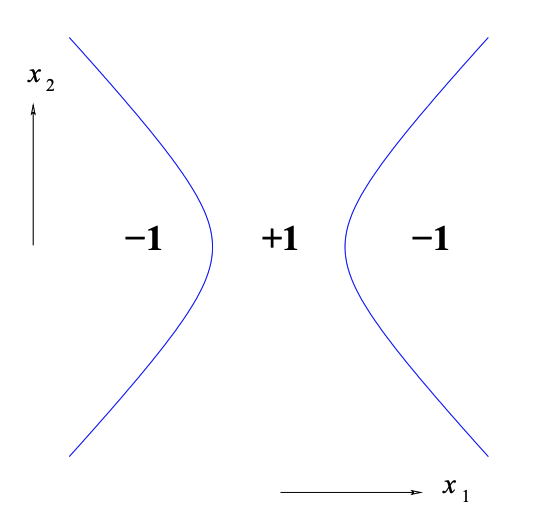
\includegraphics[width=0.32\textwidth]{img/p5-hyper.png}
\end{center}

\begin{choices}
    \choice \( \tilde{w}_1 = 0, \tilde{w}_2 > 0 \)
    \choice \( \tilde{w}_1 > 0, \tilde{w}_2 = 0 \)
    \choice \( \tilde{w}_1 > 0, \tilde{w}_2 > 0 \)
    \choice \( \tilde{w}_1 < 0, \tilde{w}_2 > 0 \)
    \choice \( \tilde{w}_1 > 0, \tilde{w}_2 < 0 \)
\end{choices}

\begin{solution}
D. \( \tilde{w}_1 < 0, \tilde{w}_2 > 0 \).

The positive classifications come from an increase in the distance
between $x_2$ and the center, while the negative classifications come
from an increase in the distance between $x_1$ and the center. 
\end{solution}

\question Consider the 4th order polynomial transform from \( \mathbb{R}^2 \):

\[
\Phi_4: \textbf{x} \rightarrow (1, x_1, x_2, x_1^2, x_1 x_2, x_2^2, x_1^3, x_1^2 x_2, x_1 x_2^2, 
x_2^3, x_1^4, x_1^3 x_2, x_1^2 x_2^2, x_1 x_2^3, x_2^4)
\]

What is the smallest value among these choices that is not smaller than the VC 
dimension of a linear model in this transformed space?

\begin{choices}
    \choice 3
    \choice 5
    \choice 15
    \choice 20
    \choice 21
\end{choices}

\begin{solution}
D. 20.

We know that $d_{\text{VC}}\le \tilde{d} + 1 \le 17$.
\end{solution}

\end{questions}

\section*{Gradient Descent}

Consider the nonlinear error surface \( E(u, v) = (u e^v - 2 v e^{-u})^2 \). 
We start at the point \( (u, v) = (1, 1) \) and minimize this error using 
gradient descent with \( \eta = 0.1 \).

\begin{verbatim}
def p5p6():
    E = lambda u, v: (u * exp(v) - 2 * v * exp(-u)) ** 2
    dEdu = lambda u, v : 2 * (u * exp(v) - 2 * v * exp(-u)) * (exp(v) + 2 * v * exp(-u)) 
    dEdv = lambda u, v : 2 * (u * exp(v) - 2 * v * exp(-u)) * (u * exp(v) - 2 * exp(-u)) 
    lr = 0.1
    u, v = 1, 1 
    iters = 0

    while E(u, v) >= 1e-14:
        u_, v_ = u, v
        u -= lr * dEdu(u_, v_)
        v -= lr * dEdv(u_, v_)
        iters += 1

    print(f"Number of iterations before error falls below 1e-14: {iters}")
    print(f"Final values for (u, v): {(u, v)}")

def p7():
    E = lambda u, v: (u * exp(v) - 2 * v * exp(-u)) ** 2
    dEdu = lambda u, v : 2 * (u * exp(v) - 2 * v * exp(-u)) * (exp(v) + 2 * v * exp(-u)) 
    dEdv = lambda u, v : 2 * (u * exp(v) - 2 * v * exp(-u)) * (u * exp(v) - 2 * exp(-u)) 
    lr = 0.1
    u, v = 1, 1 

    for _ in range(15):
        u -= lr * dEdu(u, v)
        v -= lr * dEdv(u, v)

    print(f"Final error for coordinate descent after 15 iterations: {E(u, v)}")
\end{verbatim}

\begin{questions}
\setcounter{question}{3}

\question 
What is the partial derivative \( \frac{\partial E}{\partial u} \)?

\begin{choices}
    \choice \( (u e^v - 2 v e^{-u})^2 \)
    \choice \( 2 (u e^v - 2 v e^{-u}) \)
    \choice \( 2 (e^v + 2 v e^{-u}) \)
    \choice \( 2 (e^v - 2 v e^{-u}) (u e^v - 2 v e^{-u}) \)
    \choice \( 2 (e^v + 2 v e^{-u}) (u e^v - 2 v e^{-u}) \)
\end{choices}

\begin{solution}
E. \( 2 (e^v + 2 v e^{-u}) (u e^v - 2 v e^{-u}) \)

\[
\frac{\partial E}{\partial u} = 2(ue^{v} - 2ve^{-i})(e^{v} + 2uve^{-u})
.\] 
\end{solution}

\question How many iterations (among the given choices) does it take for the 
error \( E(u, v) \) to fall below \( 10^{-14} \) for the first time? Use double 
precision in your programs to ensure accuracy.

\begin{choices}
    \choice 1
    \choice 3
    \choice 5
    \choice 10
    \choice 17
\end{choices}

\begin{solution}
D. 10
\end{solution}

\question After running enough iterations such that the error has just dropped below 
\( 10^{-14} \), what are the closest values among the following choices to the final 
\( (u, v) \) obtained?

\begin{choices}
    \choice (1.000, 1.000)
    \choice (0.713, 0.045)
    \choice (0.016, 0.112)
    \choice (-0.083, 0.029)
    \choice (0.045, 0.024)
\end{choices}

\begin{solution}
E. (0.045, 0.024)
\end{solution}

\question Now compare the performance of “coordinate descent.” In each iteration, 
there are two steps along the two coordinates. Step 1 moves only along the \( u \) 
coordinate to reduce the error (assuming a first-order approximation holds), and 
Step 2 moves only along the \( v \) coordinate. Use the same learning rate \( \eta = 0.1 \). 
What will the error \( E(u, v) \) be closest to after 15 full iterations (30 steps)?

\begin{choices}
    \choice \( 10^{-1} \)
    \choice \( 10^{-7} \)
    \choice \( 10^{-14} \)
    \choice \( 10^{-17} \)
    \choice \( 10^{-20} \)
\end{choices}

\begin{solution}
A. $10^{-1}$.
\end{solution}
\end{questions}

\section*{Logistic Regression}

In this problem you will create your own target function $f$ (probability
in this case) and data set $\mathcal{D}$ to see how Logistic Regression works.
For simplicity, we will take $f$ to be a $0 / 1$ probability so $y$ is a 
deterministic function $\textbf{x}$.

Take $d=2$ so you can visualize the problem, and let $\mathcal{X}=[-1, 1]
\times [-1,1]$ with uniform probability of picking each $\textbf{x} \in 
\mathcal{X}$. Choose a line in the plane as the boundary between $f(\textbf{x})
=1$ (where $y$ has to be $+1$) and $f(\textbf{x}) = 0$ (where $y$ has to be -1)
by taking two random, uniformly distributed points from $\mathcal{X}$ and taking
the line passing through them as the boundary between $y=\pm 1$. Pick $N=100$
training points at random from $\mathcal{X}$, and evaluate the outputs $y_{n}$
for each of these points $\textbf{x}_{n}$.

Run Logistic Regression with SGD to find $g$, and estimate $E_{\text{out}}$ (the
cross entropy error) by generating a sufficiently large, separate set of points
to evaluate the error. Repeat the experiment for 100 runs with different targets
and take the average. Initialize the weight vector of Logistic Regression to all
zeroes in each run. Stop the algorithm when $||\textbf{w}^{(t-1)}-\textbf{w}^{(t)}||
< 0.01$, where $\textbf{w}^{(t)}$ denotes the weight vector at the end of epoch
$t$. An epoch is a full pass through the $N$ data points (use a random permutation
of $1,2,\ldots,N$ to present the data points to the algorithm within each epoch,
and use different permutations for dfiferent epochs). Use a learning rate of 
$0.01$.

\begin{verbatim}
class LogReg():
    def __init__(self, dim, lr=0.01) -> None:
        self.dim = dim
        self.w = np.zeros(dim + 1)
        self.lr = lr
        self.epochs = 0

    def predict(self, x):
        x = np.concatenate((np.ones(1), x))
        s = self.w @ x
        exp = math.exp(s)
        return exp / (1 + exp)

    def step(self, x, y):
        x = np.concatenate((np.ones(1), x))
        grad = -y * x / (1 + math.exp(y * self.w @ x))
        self.w -= self.lr * grad
        return -self.lr * grad

    def sgd(self, X, Y):
        permutation = [i for i in range(X.shape[0])]
        random.shuffle(permutation)
        diff = np.zeros(self.dim + 1)
        for i in permutation:
            diff += self.step(X[i], Y[i])
        return diff

    def train(self, X, Y):
        w_diff = np.ones(self.dim + 1)
        while math.sqrt(w_diff @ w_diff) >= 0.01:
            w_diff = self.sgd(X, Y)
            self.epochs += 1

    def eval(self, X, Y):
        preds = np.array([self.predict(x) for x in X])
        for pred, y in zip(preds, Y):
            print(pred.item(), y.item())

    def error(self, X, Y):
        X = np.concat((np.ones((X.shape[0], 1)), X), axis=1)
        cross_entropy = lambda x, y: math.log(1 + math.exp(-y * self.w @ x))
        errors = [cross_entropy(x, y) for x, y in zip(X, Y)]
        return sum(errors) / len(errors)


def binary(x):
    if x < 0:
        return 0
    return 1


def rand_point():
    return np.random.uniform(-1, 1, 2)


def generate_line():
    p1 = rand_point()
    p2 = rand_point()
    m = (p2[1] - p1[1]) / (p2[0] - p1[0])
    b = p1[1] - m * p1[0]
    f = lambda x:  m * x + b
    return f


def generate_data(n, f=None):
    if f is None:
        line = generate_line()
        f = lambda x: binary(x[1] - line(x[0]))
    x = np.random.uniform(-1, 1, (n, 2))
    y = np.array([f(xi) for xi in x]).reshape((n, 1))

    return x, y


def p8p9p10():
    num_trials = 100
    num_points = 100
    epochs = []
    test_errors = []

    for _ in range(num_trials):
        line = generate_line()
        f = lambda x: binary(x[1] - line(x[0]))
        x, y = generate_data(num_points, f)
        model = LogReg(2, 0.01)
        model.train(x, y)
        # model.eval(x, y)
        epochs.append(model.epochs)

        x_test, y_test = generate_data(num_points, f)
        test_errors.append(model.error(x_test, y_test))

    print(f"Average test error: {sum(test_errors) / len(test_errors)}")
    print(f"Average epochs for training: {sum(epochs) / len(epochs)}")
\end{verbatim}

\begin{questions}
\setcounter{question}{7}

\question Which value is closest to \( E_{\text{out}} \) for \( N = 100 \)?

\begin{choices}
    \choice 0.025
    \choice 0.050
    \choice 0.075
    \choice 0.100
    \choice 0.125
\end{choices}

\begin{solution}
E. 0.125
\end{solution}

\question How many epochs does it take on average for Logistic Regression to converge 
for \( N = 100 \)? Choose the closest value.

\begin{choices}
    \choice 350
    \choice 550
    \choice 750
    \choice 950
    \choice 1750
\end{choices}

\begin{solution}
E. 1750 
\end{solution}

\end{questions}

\section*{PLA as SGD}

\begin{questions}
\setcounter{question}{9}

\question The Perceptron Learning Algorithm can be implemented as Stochastic 
Gradient Descent (SGD) using which of the following error functions \( e_n(w) \)? 
Ignore points \( w \) where \( e_n(w) \) is not twice differentiable.

\begin{choices}
    \choice \( e_n(w) = e^{-y_n w^T x_n} \)
    \choice \( e_n(w) = -y_n w^T x_n \)
    \choice \( e_n(w) = (y_n - w^T x_n)^2 \)
    \choice \( e_n(w) = \ln(1 + e^{-y_n w^T x_n}) \)
    \choice \( e_n(w) = -\min(0, y_n w^T x_n) \)
\end{choices}

\begin{solution}
E. \( e_n(w) = -\min(0, y_n w^T x_n) \)

PLA works by picking a random misclassified point and adding $y_{n}x_{n}$
to its weights. Thus, the error is the minimum between 0 and the integral
of the offset (the gradient in this case) w.r.t. the weights.
\end{solution}

\end{questions}


\end{document}
